\documentclass[11pt]{article}
\usepackage[english]{babel}
\usepackage{geometry}
\usepackage{amsmath,amsfonts,amssymb,amsthm}
\usepackage{mathtools}
\usepackage{commath}
\usepackage{graphicx}
\usepackage[utf8]{inputenc}
\usepackage{csquotes}
\usepackage{xcolor}
\usepackage[normalem]{ulem}
\usepackage{caption}
\usepackage{booktabs}
\usepackage{rotating}
\graphicspath{{figs/}}


%%%%%%%% MARGIN
\geometry{verbose, letterpaper, tmargin=3cm,
  bmargin=3cm,lmargin=2.5cm,rmargin=2.5cm}

%%%%%%%% NO PARAGRAPH INDENT
% https://tex.stackexchange.com/questions/27802/set-noindent-for-entire-file
\setlength\parindent{0pt}
\setlength{\parskip}{5pt}

%%%%%%%% SUB-FIGURE PACKAGE
\usepackage{subcaption}

%%%%%%%% HYPERREF PACKAGE
\usepackage{hyperref}
\hypersetup{linkcolor=blue}
\hypersetup{citecolor=blue}
\hypersetup{urlcolor=blue}
\hypersetup{colorlinks=true}

%%%%%%%% DEFINITION AND THEOREM DEFINITIONS
\theoremstyle{definition}
\newtheorem{definition}{Definition}[section]

\theoremstyle{remark}
\newtheorem{remark}{Remark}

\theoremstyle{remark}
\newtheorem{question}{Question}

\theoremstyle{remark}
\newtheorem{example}{Example}

\newtheorem{theorem}{Theorem}[section]

%%%%%%%% MULTI-COLUMNS PACKAGE
\usepackage{multicol}

%%%%%%%% BIB-LATEX STUFF
\usepackage[style=numeric,
            bibstyle=numeric,
            citestyle=numeric,
            hyperref=true,
            backend=biber]{biblatex}
\addbibresource{ref.bib} %Put relative path to ref

%%%%%%%% SETS DEFINITIONS
\usepackage{amssymb}
%%%% Important sets
\renewcommand{\O}{\mathbb{O}}
\newcommand{\N}{\mathbb{N}}
\newcommand{\Z}{{\mathbb{Z}}}
\newcommand{\Q}{{\mathbb{Q}}}
\newcommand{\R}{{\mathbb{R}}}

%%%% Statistics
\newcommand{\E}[1]{\mathbb{E}\left[#1 \right]}
\newcommand{\V}[1]{\mathrm{Var}\left[#1 \right]}
\renewcommand{\P}[1]{\mathrm{P}\left(#1 \right)}

%%%% Lambda Calculus Symbols
\newcommand{\dneq}{\,\, \# \,\,}
\renewcommand{\S}{\pmb{\mathrm{S}}}
\newcommand{\I}{\pmb{\mathrm{I}}}
\newcommand{\K}{\pmb{\mathrm{K}}}
\newcommand{\ch}[1]{\ulcorner #1 \urcorner}

%%%% Ordinal Lambda Calculus Symbols
\newcommand{\ordAlph}{\Sigma_{\text{Ord}}}
\newcommand{\termOrd}{\text{Term}_\text{Ord}}
\newcommand{\fl}{\mathrm{fl}}
\newcommand{\sk}{\mathrm{sk}}

%%%% Superscript to the left
% https://latex.org/forum/viewtopic.php?t=455
\usepackage{tensor}
\newcommand{\app}[3]{\tensor*[^{#1}]{\left(#2, #3\right)}{}}

%%%%%%%% LOGIC TREES
\usepackage{prftree}

%%%%%%%% SPLIT EQUATIONS
% https://tex.stackexchange.com/questions/51682/is-it-possible-to-pagebreak-aligned-equations
\allowdisplaybreaks

%%%%%%%% FLOAT SPECIFIER
% https://www.overleaf.com/learn/latex/Errors/LaTeX_Error:_Unknown_float_option_%60H%27
\usepackage{float}

%%%%%%%% ENUMERATE LABEL
% https://www.latex-tutorial.com/tutorials/lists/
\usepackage{enumitem}

%%%%%%%% CODE RENDERING !!! UNCOMMENT IF NEEDED !!!
% Compile with flag -shell-escape
%\usepackage{minted}

%%%%%%%% START DOCUMENT

\title{Evaluation of Robust Covariance Estimation for Object Detection}
%\large{Nonparametric Statistics}}
\author{Andres Felipe Tamayo-Arango \\
  aftamayoa@eafit.edu.co \and
  David Plazas Escudero \\
  dplazas@eafit.edu.co \and
  Juan Pablo Vidal-Correa \\
  jpvidalc@eafit.edu.co \and
  Juan Sebasti\'an C\'ardenas-Rodríguez \\
  jscardenar@eafit.edu.co \\[0.5cm]
  Mathematical Engineering \\
  Universidad EAFIT}
\date{\today}


\begin{document}
\maketitle

The code implemented in this paper can be found in
\href{https://bit.ly/3rQbVRQ}{this link}.

\section{Introduction}\label{sec_int}
The object detection and classification in digital images is yet a difficult challenge. This topic is a branch of a what is known as ``computer vision'' \parencite{amit20022d}. This interdisciplinary field addresses the challenge of how computers can understand and gain insight from digital images and videos, similar to how human visual system works \cite{ballard1982computer,huang1996computer,amit20022d,szeliski2010computer}. Computer vision is widely used nowadays, in application fields such as medical imaging, automotive safety, surveillance, biometrics, face detection, autonomous navigation, industrial inspection and beyond \cite{huang1996computer,szeliski2010computer}.

More specifically, object detection refers to ``anything from identifying a location to identifying and registering components of a particular object class at various levels of detail'' \parencite{amit20022d}. Object detection is a necessary requirement for the further ``recognition'' of the object or for more general tasks, such as ``tracking'' in dynamic scenarios (see \cite{li2013survey} for an excellent review in tracking methodologies). Some general object detection methodologies can be found, for example, in \cite{amit20022d,szeliski2010computer} and the references therein; for more recent developments involving deep learning, refer to \cite{jiang2018deep,zhao2019object} and the references within; finally, for an statistical approach, check \cite{li2015feature}.

This paper aims to evaluate the effectiveness of robust covariance estimations for object detection using the well-known ``region covariance'' scheme proposed in \parencite{tuzel2006}. This methodology has been widely used by different authors in different research fields \cite{wu2012real}, such as object classification/recognition \cite{hong2009sigma,sivalingam2010tensor,tosato2010multi}, human detection \cite{paisitkriangkrai2008fast,tuzel2007human,yao2007fast,hirzer2011person}, face recognition \cite{pang2008gabor,hariri20163d}, image smoothing \cite{karacan2013structure}, and object tracking \cite{porikli2006covariance,wu2008probabilistic,wu2009real,wu2009robust}.

This work is organized as follows: Section \ref{sec:just} presents a brief, but rather specific, description of three main applications of the Region Covariance approach for object detection, which serve as main justification to the purpose of this work. On other hand, Section \ref{sec:crisp} presents the general scheme for the CRISP-DM methodology for projects in analytics and describes how it is applied to the present research. Furthermore, Section \ref{sec:meth} presents the generalities on the Region Covariance method for object localization. Additionally, Section \ref{sec:res} presents the obtained results for different covariance matrix estimation and different evaluation objects. The concluding remarks and future work are discussed in Section \ref{sec:conc}.

\section{Justification}\label{sec:just}
This section briefly describes some of the most remarkable applications of the general methodology used in this work, as main justification for this exploratory work.

One of the most important applications of the methodology proposed in \parencite{tuzel2006} is in Object Tracking, which is a natural consequence of the original localization scheme. The work in \parencite{porikli2006covariance} and \parencite{wu2012real} show outstanding results for object tracking, using real-time model update. The first, uses a model update method based on Lie algebra and Lie groups to estimate the intrinsic mean of the covariance matrices through frames. The symmetric positive definite matrices $\mathrm{Sym}^+(n,\mathbb{R})$ have a Lie group structure and, hence, this approach. The table presented in Fig. \ref{fig:res_lie} shows the obtained results by the authors in different scenarios, where almost all presented good detection of the object.

\begin{figure}[H]
    \centering
    \caption{Results for experiments (taken from \cite{porikli2006covariance}).}
    \label{fig:res_lie}
    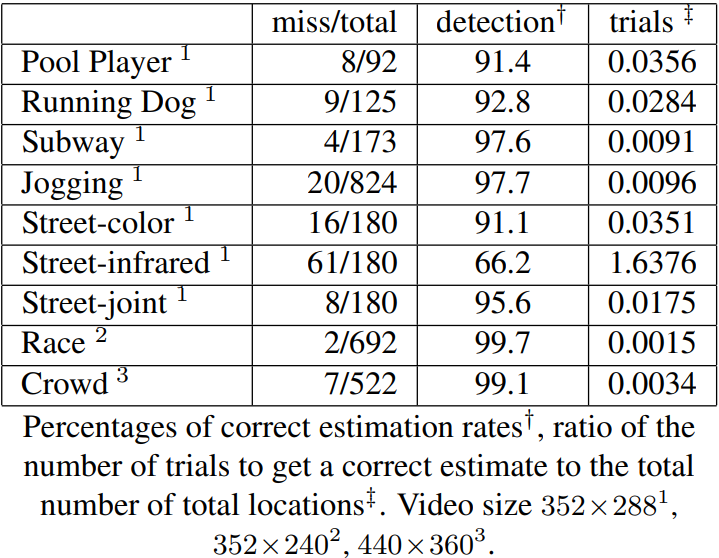
\includegraphics[scale=0.3]{res_lie.png}
\end{figure}

The second, uses a model update approach divided in two stages: a probabilistic Bayesian inference for covariance tracking $-$ via Maximum A Posteriori (MAP) estimation $-$, and an Incremental Covariance Tensor Learning (ICTL). The former propagates the sample distribution over time and the latter learns a low-dimensional covariance model online, as time progresses. The general scheme of this approach is presented in Fig. \ref{fig:scheme}. The authors claim to have achieved real-time performance using state-of-the-art data structures for images.

\begin{figure}[H]
    \centering
    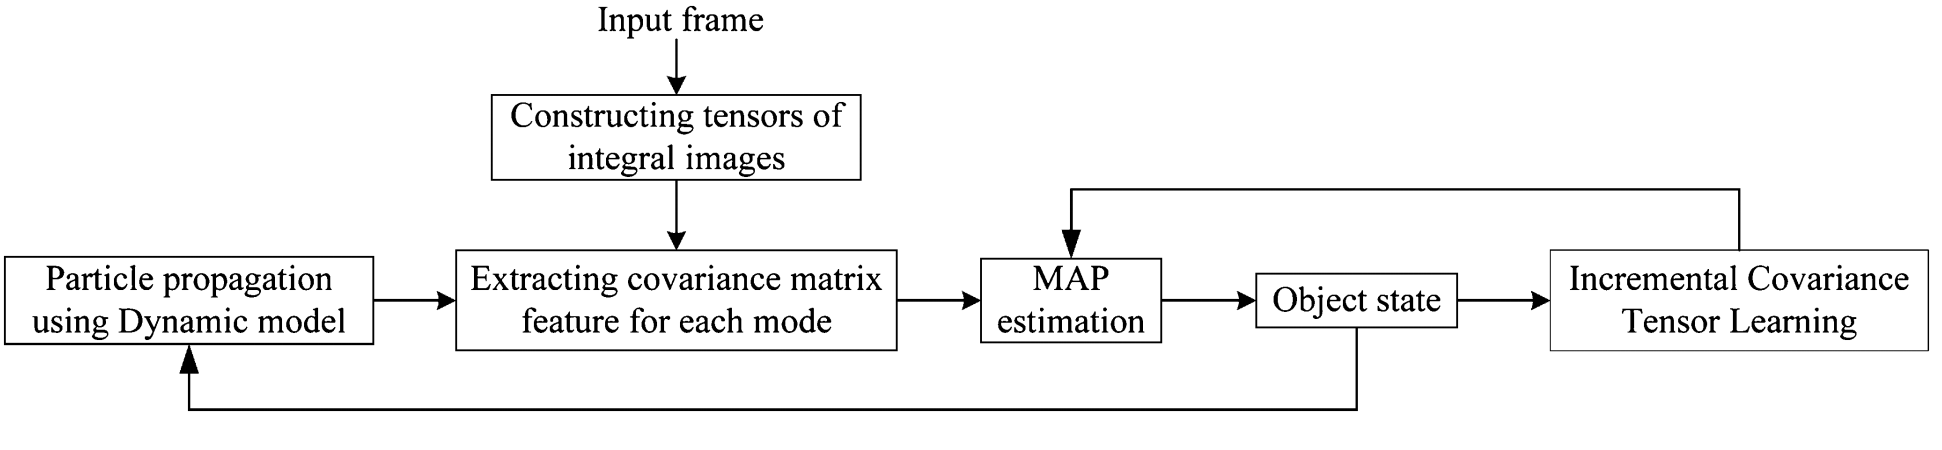
\includegraphics[scale=0.21]{scheme.png}
    \caption{General scheme (taken from \parencite{wu2012real}).}
    \label{fig:scheme}
\end{figure}


The work presented in \cite{pang2008gabor} shows a newly developed feature descriptor framework, deeply related with Region Covariance Matrices (RCMs) to perform face recognition. The use of RCMs provides a natural method of fusing multiple features in addition to the fact that RCM has a low dimension, and it is independent from scale or illumination. The table presented in Fig. \ref{fig:accuracy} shows the obtained results by the authors comparing the accuracy of face recognition between RCM-based methods and classical methods such as principal component analysis (PCA), linear discriminant analysis (LDA), kernel PCA (KPCAP) and kernel LDA (KLDA). Note that, although the normal RCM performs poorly, the Gabor-based RCM outperforms the standard methods, giving better accuracy.

\begin{figure}[H]
    \centering
    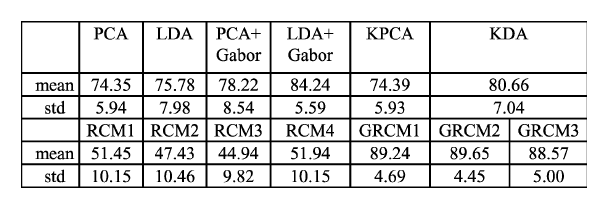
\includegraphics[scale = 0.45]{accuracy_comparing.png}
    \caption{Results of accuracy (taken from \cite{pang2008gabor})}
    \label{fig:accuracy}
\end{figure}

Finally, the work developed in \parencite{porikli2006robust} shows a remarkable application for detection of license plates using the covariance as region descriptor and then it is flatten into an input vector to a multi-layer perceptron (faster than calculating the dissimilarities between the matrices). The authors claim that this approach is robust against noises, illumination distortions and rotations. In Fig. \ref{fig:plate}, an example of covariance matrix estimation from a 7-feature vector per pixel. Furthermore, Fig. \ref{fig:roc} shows the estimated ROC curve for 4 different experiments, using a different method and different feature vectors.

\begin{figure}[H]
    \centering
    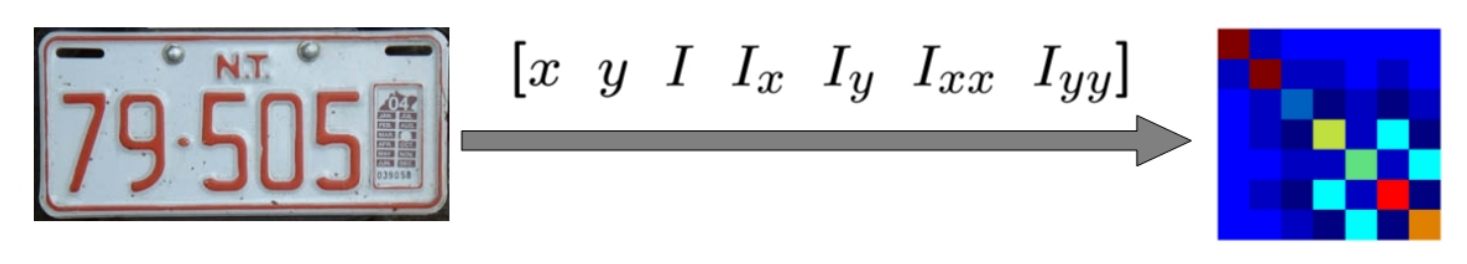
\includegraphics[scale=0.2]{plate.png}
    \caption{Example of covariance matrix from features (taken from \parencite{porikli2006robust}).}
    \label{fig:plate}
\end{figure}

\begin{figure}[H]
    \centering
    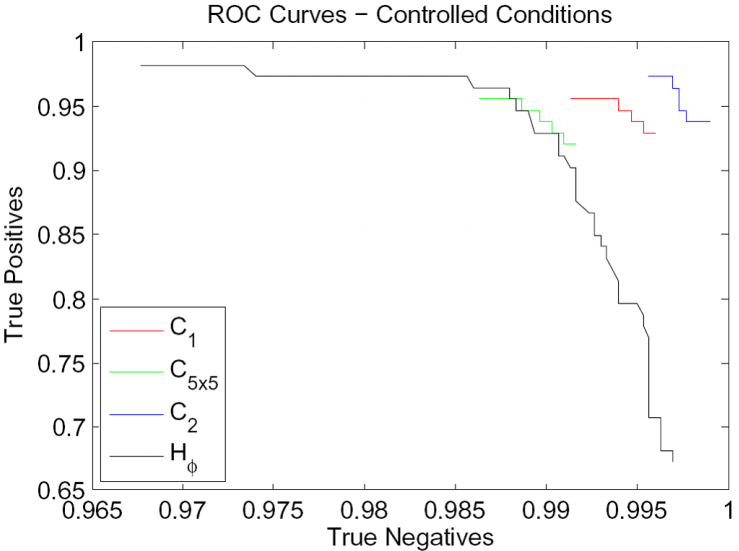
\includegraphics[scale=0.3]{roc.png}
    \caption{ROC curve for different feature vectors (taken from \parencite{porikli2006robust}).}
    \label{fig:roc}
\end{figure}

\section{CRISP-DM Methodology}\label{sec:crisp}
The CRISP-DM (Cross Industry Standard Process for Data Mining) methodology splits the data-mining endeavor into six phases: business understanding, data understanding, data preparation, modeling, evaluation and deployment \cite{Chapman2000CRISPDM1S}. 

\begin{figure}[H]
    \centering
    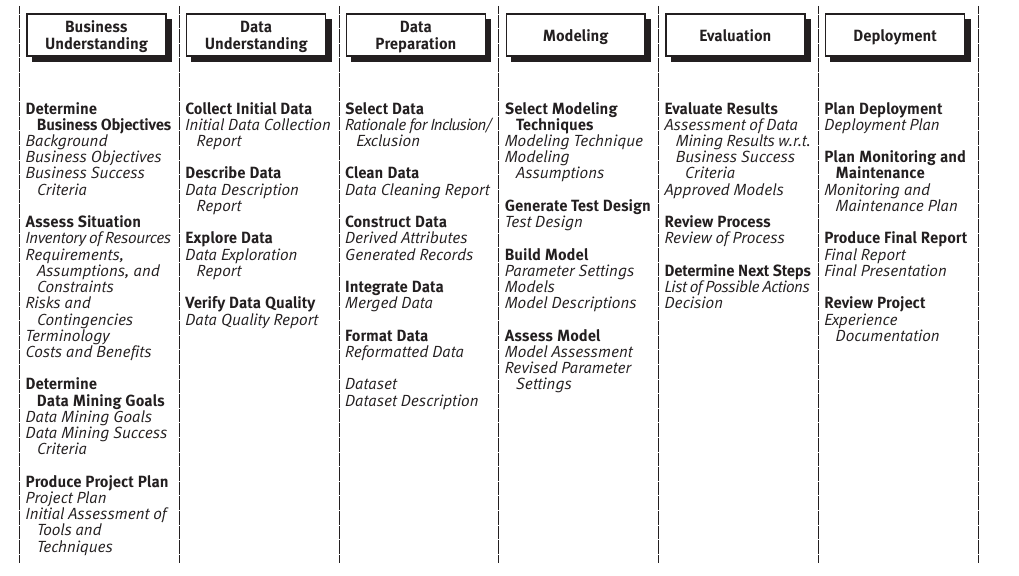
\includegraphics[width = 0.8\linewidth]{crisp-dm.png}
    \caption{CRISP-DM Methodology (taken from \cite{Chapman2000CRISPDM1S}).}
    \label{fig:crisp-dm}
\end{figure}

\textbf{Business Understanding:} \textit{The first objective of the data analyst is to thoroughly understand, from a business perspective, what the
customer really wants to accomplish. Often the customer has many competing objectives and constraints
that must be properly balanced. The analyst’s goal is to uncover important factors, at the beginning, that
can influence the outcome of the project.}

For the phase of Business Understanding see sections \ref{sec_int} and \ref{sec:just}.

\textbf{Data Understanding:} \textit{Acquire the data (or access to the data) listed in the project resources. This initial collection includes data loading, if necessary for data understanding.}

The acquire data for the project were personal photos for the following reasons.
The input object was required to have different scale, orientation, location, and lighting characteristics in order to evaluate performance with the different metrics and covariance estimates. On the other hand, it is necessary to be able to manually locate the real object to assess the correct location of the object (supervise focus).

\textbf{Data Preparation:} \textit{These are the dataset(s) produced by the data preparation phase, which will be used for modeling or the
major analysis work of the project.}

For current project the data preparation phase was developed as follows. In the first step we take six photos of an object, one of this is considered as the input of the program and the other five were considered as test cases. This last photo was cropped in order to become into a single image. On the other hand, all images were scaled so that their major axis had 70 pixels. Finally, real objects were extracted from the five test images for further evaluation of the program.

\textbf{Modeling:} \textit{As the first step in modeling, select the actual modeling technique that is to be used. Although you may have already selected a tool during the Business Understanding phase, this task refers to the specific
modeling technique, e.g., decision-tree building with 5.0, or neural network generation with back
propagation. If multiple techniques are applied, perform this task separately for each technique. }

For modeling phase, see section \ref{sec:meth}.

\textbf{Evaluation:} \textit{This step
assesses the degree to which the model meets the business objectives and seeks to determine if there is
some business reason why this model is deficient. Another option is to test the model(s) on test applications
in the real application, if time and budget constraints permit}

For Evaluation phase, see section \ref{sec:res}

\textbf{Deployment:} \textit{This task takes the evaluation results and determines a strategy for deployment. If a general procedure has
been identified to create the relevant model(s), this procedure is documented here for later deployment.}

Deployment phase can be found in \href{https://github.com/Daples/JuanSePlazas/tree/master/202/algebra-in-data-science/final-project}{this link}.


\section{Methodology}\label{sec:meth}

\subsection{Covariance as a Region Descriptor}

Descriptors are set of numbers produced to describe a given shape in a quantifiable measure \parencite{tyagi2018content}. The shape may not be entirely reconstructed from the descriptors, but these measures for different shapes should be different enough that the shapes can be discriminated \cite{cui2013fusing}. A region descriptor describes the object within based on the pixel distribution in this 2‐D array.

The covariance as a region descriptor, proposed in \parencite{tuzel2006}, will now be presented. For an image of width $W$ and height $H$, let $\mathcal{W}=\{1,\ldots,W\}$ and $\mathcal{H}=\{1,\ldots,H\}$. The image is then mapped into a feature space for each pixel
\[
    F:\mathcal{W}\times\mathcal{H}\rightarrow\mathbb{R}^{d}
\]
yielding a tensor $\mathcal{A} \subset \R^{W \times H \times d}$, as depicted in Fig. \ref{fig:feat_ext}.
\begin{figure}[H]
    \centering
    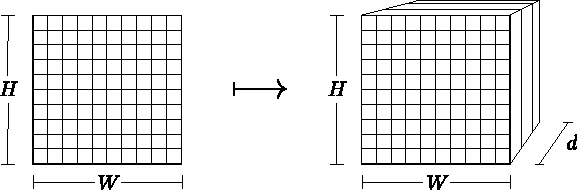
\includegraphics[width = 0.6\linewidth]{figs/feature_extraction.pdf}
    \caption{Feature extraction.}
    \label{fig:feat_ext}
\end{figure}
%
Let $W'$ and $H'$ the width and height of region $R\subset\mathcal{A}$. The covariance matrix of $R$ is estimated by flattening the region into a $(W'\cdot H')\times d$ data matrix, yielding $\mathbf{C}_R \in \R^{d \times d}$. This process is depicted in Fig. \ref{fig:region}.
\begin{figure}[H]
    \centering
    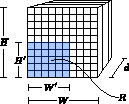
\includegraphics[width = 0.3\linewidth]{figs/region1.pdf}
    \caption{Region tensor.}
    \label{fig:region}
\end{figure}

There are multiple advantages for using the covariance as a region descriptor. Usually, a single covariance matrix extracted from a region is enough to match the region in different views, since the covariance of a distribution is enough to discriminate it from other distributions. Moreover, the covariance matrix allows to observe features that might be correlated and filter out noise corrupting samples during the computation.

Additionally, the covariance matrices are low-dimensional, compared to other region descriptors and due to symmetry $\mathbf{C}_{R}$ has only $\left(d^{2}+d\right) / 2$ different values. This method also allows to discriminate orientation, scale and illumination features from an image, since the covariance descriptor is not invariant regarding the orientation of the points.

\subsection{Metrics}
\begin{definition}
The matrix norm is a function $\norm{\cdot}: \mathbf{K}^{m \times n} \to \R$ where $\mathbf{K}$ is the set of either real or complex numbers and $\mathbf{K}^{m \times n}$ is the vector space of all matrices of size $m \times n$. This function must satisfies the following five axioms:
\begin{enumerate}
    \item $\norm{\mathbf{A}} \geq 0$
    \item $\norm{\mathbf{A}} = 0$ if and only if $\mathbf{A} = 0$
    \item $\norm{c\mathbf{A}} = |c|\norm{\mathbf{A}}$
    \item $\norm{\mathbf{A} + \mathbf{B}} \leq \norm{\mathbf{A}} + \norm{\mathbf{B}}$
    \item $\norm{\mathbf{AB}} \leq \norm{\mathbf{A}}\norm{\mathbf{B}}$
\end{enumerate}
\end{definition}

\begin{example}
The $l_{1}$ norm is defined for $\mathbf{A} \in \mathbf{K}^{m \times n}$ by
%
\[
\norm{\mathbf{A}}_{1} = \sum_{i,j = 1}^{n} |a_{ij}|
\]
\end{example}

\begin{example}
The $l_{\infty}$ norm is defined for $\mathbf{A} \in \mathbf{K}^{m \times n}$ by 
%
\[
\norm{\mathbf{A}}_{\infty} = \max_{i}{\sum_{j = 1}^{n} |a_{ij}|}
\]

\end{example}

\subsubsection{Frobenius}
An $M \times N$ matrix $\mathbf{A}$ can be consider as a particular kind of vector $x = \mathbf{A} \in \R^{m,n}$, and its norm is any function that maps $\mathbf{A}$ to a real number $\norm{\mathbf{A}}$. In this order of ideas, if we treat the $M \times N$ elements of $\mathbf{A}$ as the elements of an $MN-$dimensional vector, then the $p-$norm of this vector can be used as the $p-$norm of $\mathbf{A}$:
%
\[
\norm{\mathbf{A}}_{p} = \left\{ \sum_{i = 1}^{M} \sum_{j=1}^{N} \lvert a_{ij} \rvert^{p} \right\}^{1/p}
\]
%
If we consider the case when $p = 2$ we got the Frobenius norm $\norm{\mathbf{A}}_{F}$
%
\[
\norm{\mathbf{A}}_{2} = \norm{\mathbf{A}}_{F} = \sqrt{\sum_{i=1}^{M} \sum_{j=1}^{N} \lvert a_{ij} \rvert^{2}} = \sqrt{\mathrm{tr}(\mathbf{A}^{T}\mathbf{A})}
\]

\subsubsection{Dissimilarity of Two Covariance Matrices} \label{subsub:dis}

It is well known that the covariance matrix lies on a non-euclidean space, therefore, in order to measure the dissimilarity of two covariance matrices, the distance measure proposed in \parencite{forstner2003metric} is used:
%
\begin{equation}\label{eq:3}
\rho\left(\mathbf{C}_{1}, \mathbf{C}_{2}\right)=\sqrt{\sum_{i=1}^{n} \ln ^{2} \lambda_{i}\left(\mathbf{C}_{1}, \mathbf{C}_{2}\right)}
\end{equation}
%
where $\left\{\lambda_{i}\left(\mathbf{C}_{1}, \mathbf{C}_{2}\right)\right\}_{i=1}^n$ are the generalized eigenvalues of $\mathbf{C}_{1}$ and $\mathbf{C}_{2},$ computed from
%
\[
\lambda_{i} \mathbf{C}_{1} \mathbf{x}_{i}-\mathbf{C}_{2} \mathbf{x}_{i}=0, \quad i=1 \ldots d
\]
%
and $\mathbf{x}_{i} \neq 0$ are the \textbf{generalized eigenvectors}. The distance measure $\rho$ satisfies the metric axioms for positive definite symmetric matrices (see \parencite{tuzel2006}). The equation (\ref{eq:3}) can be computed with a $O\left(d^{3}\right)$ arithmetic operations using numerical methods.
\subsection{Covariance Computation}
  
The methods for estimating the covariance matrix of each image region will be now presented:

\subsubsection{Maximum Likelihood Estimation}

The maximum likelihood estimation (with the unbiased correction factor) of this covariance matrix is given by
%
\begin{equation}
\mathbf{C}_{R}=\frac{1}{n-1} \sum_{k=1}^{n}\left(\mathbf{z}_{k}-\boldsymbol{\mu}\right)\left(\mathbf{z}_{k}-\boldsymbol{\mu}\right)^{T}
\end{equation}
%
where $\boldsymbol{\mu}$ is the mean vector of the features inside the region.

\subsubsection{Comedian Estimation}

The first robust calculation of the distance is based on a robust estimation of the
covariance matrix following the ideas from \parencite{falk1997mad}, using the following definition.

Let $X$ and $Y$ be two random vectors. The comedian between $X$ and $Y$ is defined as
%
\[
\operatorname{Com}(X, Y)=\operatorname{Med}[(X-\operatorname{Med}(X))(Y-\operatorname{Med}(Y))].
\]
%
The covariance matrix is then estimated by applying the comedian to each feature of the data (comedian matrix). 

\subsubsection{Kendall Estimation}

This method uses the Kendall rank correlation coefficient, usually known as Kendall's $\tau$ coefficient, originally proposed in \parencite{kendall1938new}. In order to define the Kendall's $\tau$ coefficient we have to give a notion of concordance. 

\begin{definition}
Let $(x_{j},y_{j})$ and $(x_{k},y_{k})$ be two elements of a sample $\{(x_{i},y_{i})\}_{i=1}^{n}$ from a bivariate population. One says that $(x_{j},y_{j})$ and $(x_{k},y_{k})$ are \textit{concordant} if 
\[
x_{j} < x_{k} \quad \text{and} \quad y_{j} < y_{k}
\]
or if
\[
x_{j} > x_{k} \quad \text{and} \quad y_{j} > y_{k}
\]
On the other hand, $(x_{j},y_{j})$ and $(x_{k},y_{k})$ are \textit{discordant} if
\[
x_{j} < x_{k} \quad \text{and} \quad y_{j} > y_{k}
\]
or if
\[
x_{j} > x_{k} \quad \text{and} \quad y_{j} < y_{k}
\]
\end{definition}

Given this definition and establishing that the number of distinct pairs of observations in the sample is given by $\binom{n}{2}$ and each pair is either concordant or discordant one can denote as $S$ the number of concordant pairs minus the number of discordant pairs and give the definition of the Kendall's $\tau$ for the sample as 

\[
\tau = \dfrac{S}{\binom{n}{2}} = \dfrac{2S}{n(n-1)}
\]

With this coefficient, each entry of the covariance matrix is estimated using
\[
\operatorname{Cov}(x, y)=\rho_{k} S_{x} S_{y}
\]
where $\rho_{k}$ is Kendall's $\tau$ coefficient, and $S_{x}$ and $S_{y}$ are the respective standard deviations.

\subsection{Spearman Estimation}

This estimation was performed similarly to Kendall's. The covariance matrix is estimated using
\[
\operatorname{Cov}(x, y)=\rho_{s} S_{x} S_{y}
\]
where $\rho_{s}$ is Spearman's correlation coefficient (see \parencite{spearman1961general}), and $S_{x}$ and $S_{y}$ are the respective standard deviations. Spearman's coefficient can be defined as follows (see \cite{spearmscoeff}). Suppose that there are $n$ pairs of associated rankings
\[
u_{1}, u_{2}, \ldots, u_{n} \quad \text{and} \quad v_{1}, v_{2}, \ldots, v_{n} 
\]
where the integers $u_{i}$ $(i = 1,2,\ldots,n)$ may be taken in ascending order $1,2,\ldots,n$ and the $v_{i}$ are a permutation of these integers. The measure of correlation between these rankings given by the Spearman's coefficient is simply the product moment correlation coefficient of $u_{i}$, $v_{i}$ and may be computed from the sum of squared differences
\[
S_{s} = \sum_{i = 1}^{n} (u_{i} - v_{i})^{2} 
\]
Then, the coefficient is given by
\[
\rho_{s} = 1 - \dfrac{6S_{s}}{n^{3} - n}
\]
\textbf{Ledoit and Wolf Estimation}

This method, proposed in \parencite{ledoit2004honey}, uses the shrinkage constant $\delta$, to ‘shrunk’ the sample covariance matrix towards the structured estimator. The covariance matrix is estimated using

\[
\operatorname{Cov}(x, y)={\delta} F+\left(1-{\delta}\right)S
\]

where $S$ is the sample covariance matrix, $F$ is a structured estimator and $\delta$ is a number between 0 and 1. 


\subsection{Object Detection}
Based on the methodology proposed in \parencite{tuzel2006} for object detection, the following approach is used to locate an object image in an arbitrary image after a nonrigid transformation.

Initially, the location of a pixel in the target image is defined by its coordinates $(x,y)$. The axis coordinates define the pixel location as an array in multi-dimensional space. Each image axis has a length, in pixels, so that the image coordinates run between 1 and the length of the axis \parencite{mikhail1984detection}. Then, each pixel of the image is converted to a nine-dimensional feature vector
%
\begin{equation}
F(x, y)=\left[x,\, y,\, R(x, y),\, G(x, y),\, B(x, y),\,\left|\frac{\partial I(x, y)}{\partial x}\right|,\,\left|\frac{\partial I(x, y)}{\partial y}\right|,\,\left|\frac{\partial^{2} I(x, y)}{\partial x^{2}}\right|,\,\left|\frac{\partial^{2} I(x, y)}{\partial y^{2}}\right|\right]^{T}
\end{equation}
%
with RGB color values, and intensity $I$. The first and second order derivatives are calculated through Sobel filters.

The first step is to estimate the covariance matrix of the input target object $T$. A brute force search is performed to find matching regions, analyzing nine different scales (four smaller, four larger). Instead of scaling the target image, the size of the search window is varied with a 15\% scaling factor between two consecutive scales. 

After the search, the best matching 1000 locations are kept and each region is divided into five different subregions to evaluate different covariances of the region; this division is better depicted in Fig. \ref{fig:regions}.

\begin{figure}[H]
    \centering
    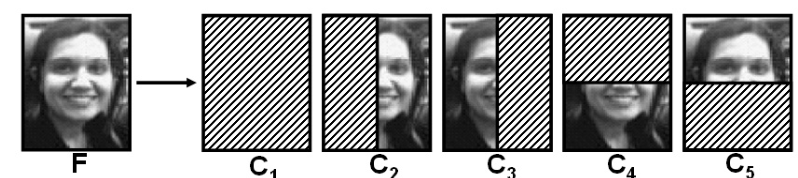
\includegraphics[scale=.6]{figs/regions.png}
    \caption{Region subdivision, image taken from \parencite{tuzel2006}.}
    \label{fig:regions}
\end{figure}

Finally, the objective function is evaluated to find the matching region. The idea behind this function is find the region $R$ that minimizes the dissimilarity of itself with all the remaining:

\begin{equation*}
    \lambda(R, T)=\min _{j}\left[\sum_{i=1}^{5} \rho\left(\mathbf{C}_{i}^{R}, \mathbf{C}_{i}^{T}\right)-\rho\left(\mathbf{C}_{j}^{R}, \mathbf{C}_{j}^{T}\right)\right]
\end{equation*}

where $\mathbf{C}_j^R$ is the $j$-th covariance matrix from Fig. \ref{fig:regions} for the region $R$ and $\mathbf{C}_j^T$ is the $j$-th covariance matrix of the target object.

\subsection{Performance Measures}
For each of the test cases the expected result was extracted to measure the performance of the algorithms. In this manner, two performance measures of each of the test cases were calculated, the value of the objective function and the distance between the covariance matrix of the expected result and the algorithm result. This measures allowed to understand how close the algorithm was to obtaining the correct result and how well the optimization problem was solved.

It is important to remark than metrics, normally, have a wide range of scales between them. This generated difficulties in the way to compare them. To solve this issue, to compare each of the dissimilarity functions the distance to the original object for each of the test cases is were used. The idea was to see if, normally, one of the dissimilarity function outperformed (had a smaller distance to the original) than the other one. Hence, a linear regression of this distances were extracted using the desired metrics. If the linear regression is significant, this would allow to see which metric had a more close result to the expected one. The distance explained in Subsection \ref{subsub:dis} was used for calculating the distance between the expected and the algorithm result.

On the other hand, for comparing each of the covariances a similar strategy was used. Let $n$ be the number of test cases. For each covariance matrix $i$ and distance $j$ a matrix $M_{ij} \in \R^{n\times2}$ was constructed containing the value of the objective function and the distance to the expected result. Then a scatter plot was constructed for each of distance $j$ to see which covariance matrix, generally, minimized both of the performance metrics. As both of the performance measures are desired to be minimized, a pareto curve is obtained in order to solve the multi-objective optimization problem.

\section{Results}\label{sec:res}
This work only presents some localization results that the authors considered valuable for the discussion and concluding remarks. The complete output for all possible 500 combination of covariance matrices, type of input and metric can be found in \href{https://bit.ly/2VMkvne}{this link}. This zipped file contains several folders, one for each input image with its respective test cases. All files follow an standardized name structure: \texttt{noise-cov-dist-test\_caseX.jpg} where

\begin{table}[H]
\centering
\begin{tabular}{llllll}
\texttt{noise}: & 0 $\rightarrow$ Impulse  & \texttt{cov}: & 0 $\rightarrow$ MLE      & \texttt{dist}: & 0 $\rightarrow$ Author    \\
                & 1 $\rightarrow$ No noise &               & 1 $\rightarrow$ Comedian &                & 1 $\rightarrow$ Frobenius \\
                &                          &               & 2 $\rightarrow$ Spearman &                &                           \\
                &                          &               & 3 $\rightarrow$ Kendall  &                &                           \\
                &                          &               & 4 $\rightarrow$ LW       &                &                          
\end{tabular}
\end{table}

\subsection{Implementation}
This section briefly describes some details of the implementation of the algorithm. First, we calculate the first and second order derivatives of all pixels in both the input and target images, instead of calculating on each region considered; this allows the implementation to access the derivatives for each region, used in the features, in constant time. Second, the whole methodology was tested using RGB color scheme. Third, an additional step was included in the detection process: the ``transpose'' of the region is also considered in search for a matching region; this allows the algorithm to detect possible rotations of the image or object in question by switching the width and height of the searching region.

\subsection{Implementations}
In Table \ref{tab:times}, the execution time in seconds and the mega-bytes consumed by the implementations can be found. The ``naïve'' implementation used \texttt{for}-loops and suggested commands to find each of the estimators. The ``ours'' implementation used only matrix operations. This was tested with a uniform random matrix of size $1000\times 500$ once, as one run is enough to compare the speeds as calculating a similar sized matrix rarely varies in execution time.
%
\begin{table}[H]
    \centering
    \begin{tabular}{cccc}
        \hline
                   & Spearman      & Kendall       & Comedian      \\
        Na\"ive (s)  & 1.44          & 162.13        & 369.78        \\
        Ours (s)   & \textbf{0.30} & \textbf{4.11} & \textbf{3.66} \\
        Na\"ive (MB) & \textbf{109}  & \textbf{108}  & \textbf{104}  \\ 
        Ours (MB)  & 115           & 1977          & 2020    \\     \hline
    \end{tabular}
    \caption{Tests with random matrix in $\R^{1000\times500}$.}
    \label{tab:times}
\end{table}

\subsection{Image Results with Kendall Matrix}
Some examples of the object localization results, for different input objects, are presented in Figs. \ref{fig:test_rubik_aut}-\ref{fig:test_deer_fro}. These results only present locations obtained with the Kendall covariance matrix, varying the metric and for input with and without noise. 
\begin{figure}[H]
  \centering
  \begin{subfigure}[b]{0.32\textwidth}
    \centering
    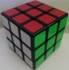
\includegraphics[width=\textwidth]{figs/input2.jpg}
    \caption{Input.}
  \end{subfigure}
  \begin{subfigure}[b]{0.32\textwidth}
    \centering
    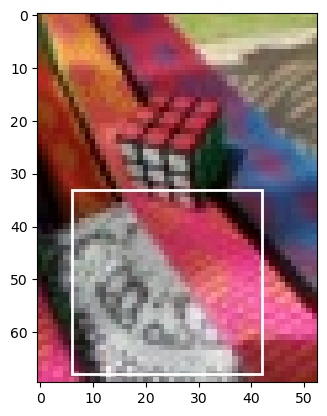
\includegraphics[width=\textwidth]{figs/0-3-0-test_case4.jpg}
    \caption{With noise.}
  \end{subfigure}
  \begin{subfigure}[b]{0.32\textwidth}
    \centering
    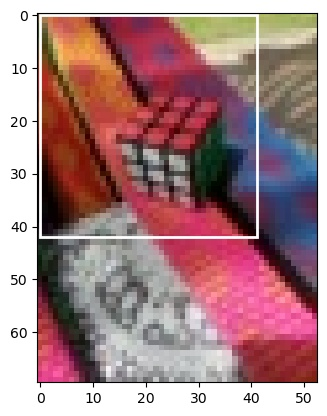
\includegraphics[width=\textwidth]{figs/1-3-0-test_case4.jpg}
    \caption{Without noise.}
  \end{subfigure}
  \caption{Tests for Rubik's cube with authors' metric.}
  \label{fig:test_rubik_aut}
\end{figure}

\begin{figure}[H]
  \centering
  \begin{subfigure}[b]{0.32\textwidth}
    \centering
    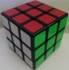
\includegraphics[width=\textwidth]{figs/input2.jpg}
    \caption{Input.}
  \end{subfigure}
  \begin{subfigure}[b]{0.32\textwidth}
    \centering
    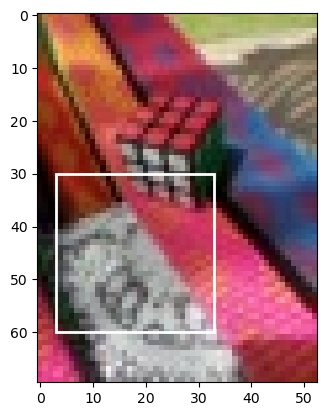
\includegraphics[width=\textwidth]{figs/0-3-1-test_case4.jpg}
    \caption{With noise.}
  \end{subfigure}
  \begin{subfigure}[b]{0.32\textwidth}
    \centering
    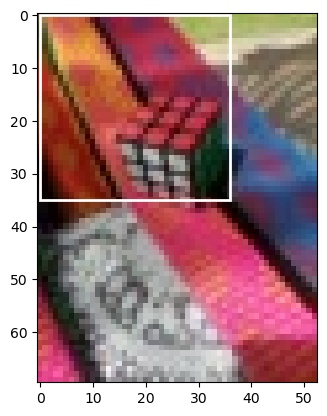
\includegraphics[width=\textwidth]{figs/1-3-1-test_case4.jpg}
    \caption{Without noise.}
  \end{subfigure}
  \caption{Tests for Rubik's cube with Frobenius metric.}
  \label{fig:test_rubik_fro}
\end{figure}

\begin{figure}[H]
  \centering
  \begin{subfigure}[b]{0.32\textwidth}
    \centering
    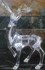
\includegraphics[width=\textwidth]{figs/input3.jpg}
    \caption{Input.}
  \end{subfigure}
  \begin{subfigure}[b]{0.32\textwidth}
    \centering
    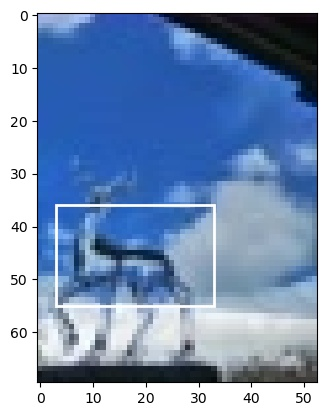
\includegraphics[width=\textwidth]{figs/0-3-0-test_case3.jpg}
    \caption{With noise.}
  \end{subfigure}
  \begin{subfigure}[b]{0.32\textwidth}
    \centering
    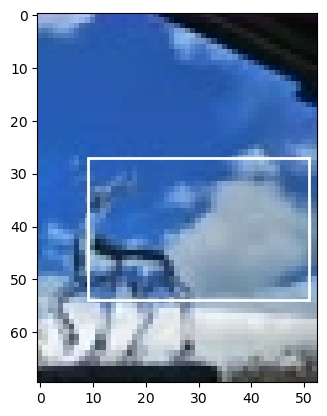
\includegraphics[width=\textwidth]{figs/1-3-0-test_case3.jpg}
    \caption{Without noise.}
  \end{subfigure}
  \caption{Tests for glass deer with authors' metric.}
  \label{fig:test_deer_aut}
\end{figure}

\begin{figure}[H]
  \centering
  \begin{subfigure}[b]{0.32\textwidth}
    \centering
    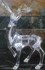
\includegraphics[width=0.9\textwidth]{figs/input3.jpg}
    \caption{Input.}
  \end{subfigure}
  \begin{subfigure}[b]{0.32\textwidth}
    \centering
    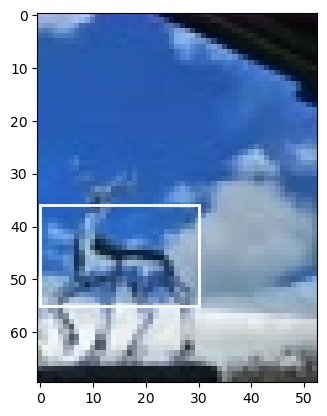
\includegraphics[width=\textwidth]{figs/0-3-1-test_case3.jpg}
    \caption{With noise.}
  \end{subfigure}
  \begin{subfigure}[b]{0.32\textwidth}
    \centering
    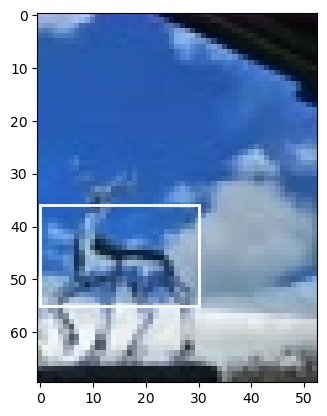
\includegraphics[width=\textwidth]{figs/1-3-1-test_case3.jpg}
    \caption{Without noise.}
  \end{subfigure}
  \caption{Tests for glass deer with Frobenius metric.}
  \label{fig:test_deer_fro}
\end{figure}

\subsection{Image Results with LW}
In Fig. \ref{fig:test_bike_lw}, the localization of noisy input images is presented, using the Ledoit and Wolf covariance matrix estimation. Note that the authors metric shows better results.
\begin{figure}[H]
  \centering
  \begin{subfigure}[b]{0.32\textwidth}
    \centering
    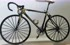
\includegraphics[width=\textwidth]{figs/input4.jpg}
    \caption{Input.}
  \end{subfigure}
  \begin{subfigure}[b]{0.32\textwidth}
    \centering
    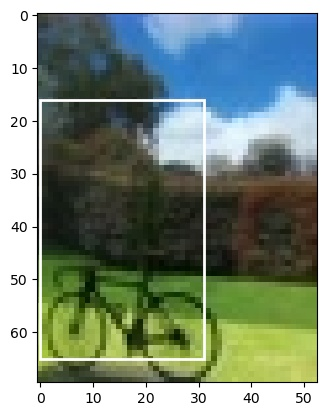
\includegraphics[width=\textwidth]{figs/0-4-0-test_case1.jpg}
    \caption{Authors' metric.}
  \end{subfigure}
  \begin{subfigure}[b]{0.32\textwidth}
    \centering
    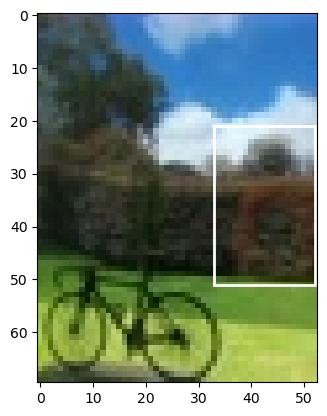
\includegraphics[width=\textwidth]{figs/0-4-1-test_case1.jpg}
    \caption{Frobenius metric.}
  \end{subfigure}
  \caption{Tests for bike with noise.}
  \label{fig:test_bike_lw}
\end{figure}

\subsection{Metrics}
As can be appreciated in the Fig. \ref{fig:linear}, the metrics were compared by setting a scatter plot of the distances to the real covariance matrix, using the Frobenius and the authors' dissimilarity measures:

\begin{figure}[H]
    \centering
    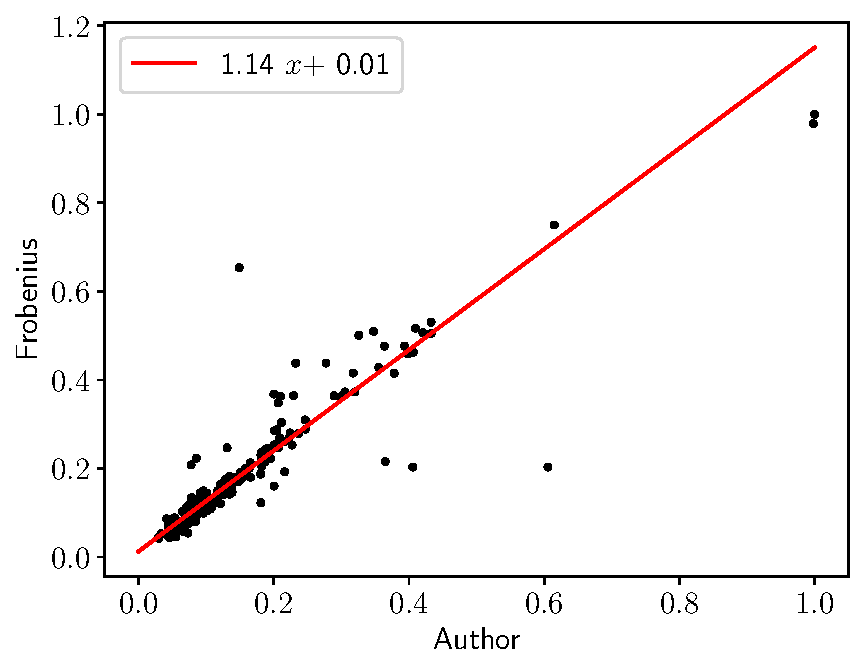
\includegraphics[width=0.6\textwidth]{figs/linear.pdf}
    \caption{Linear regression comparing metrics.}
    \label{fig:linear}
\end{figure}

\subsection{Covariance Matrices}

In Figs. \ref{fig:paretocova} and \ref{fig:paretocovf}, the Pareto boundaries for covariance matrices using the author's metric and the Frobenius metric, are presented. Note that both cases present a boundary determined only by points obtained using Kendall's covariance matrix, suggesting that this estimation is overall better.

\begin{figure}[H]
    \centering
    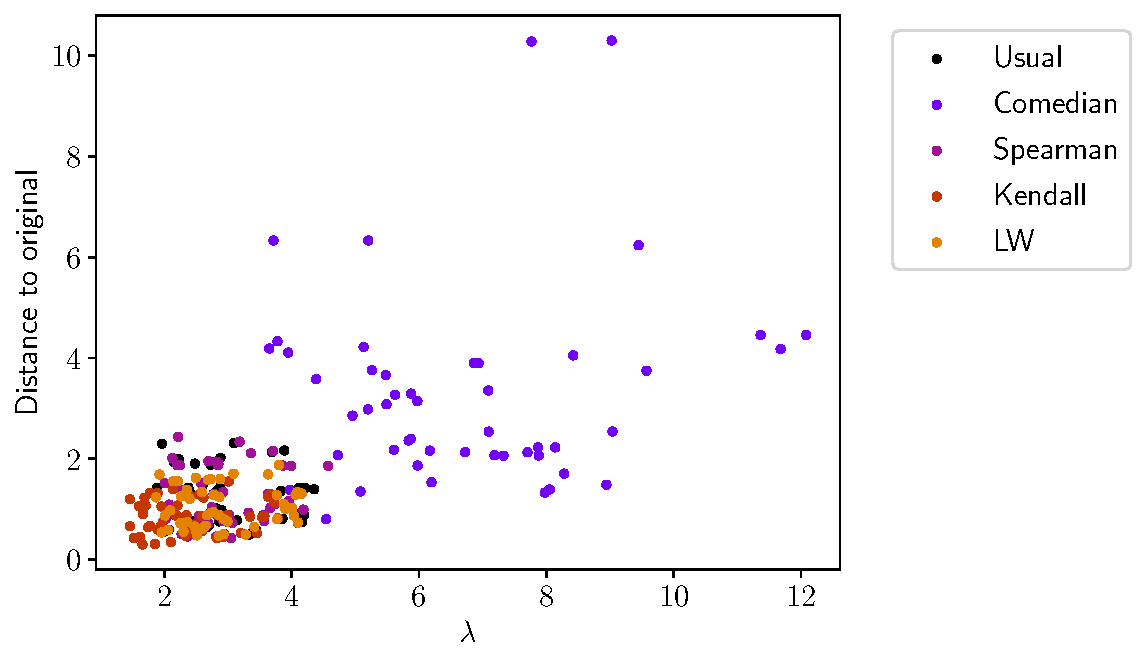
\includegraphics[width=0.8\textwidth]{figs/author-scatter.pdf}
    \caption{Pareto boundaries for covariance matrices (authors' metric).}
    \label{fig:paretocova}
\end{figure}

\begin{figure}[H]
    \centering
    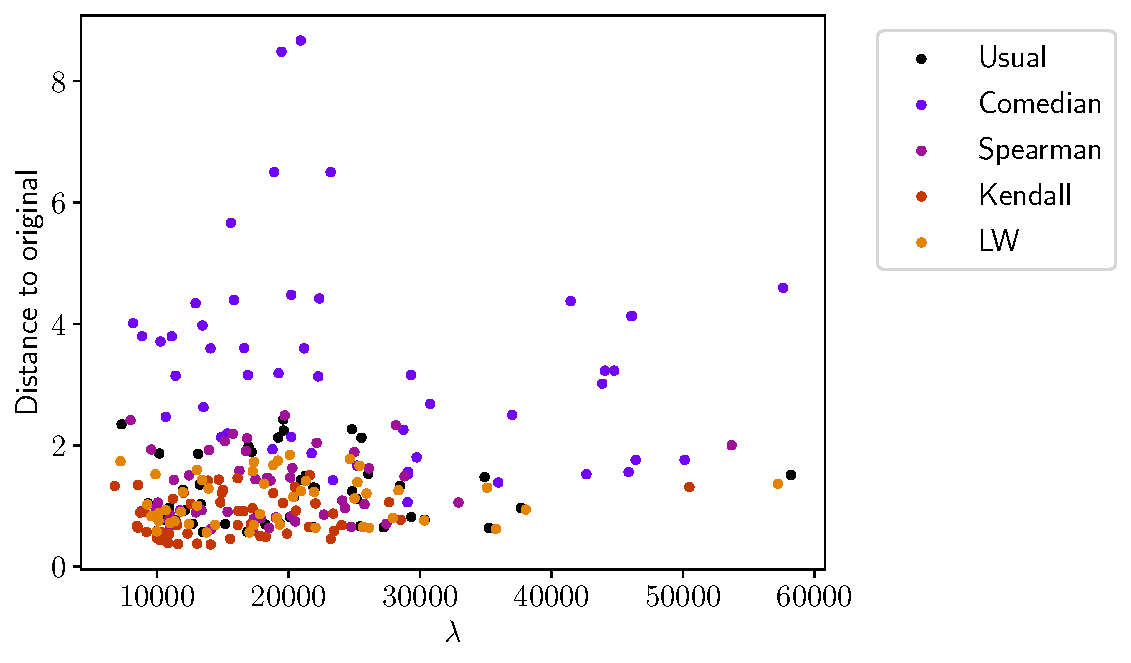
\includegraphics[width=0.8\textwidth]{figs/fro-scatter.pdf}
    \caption{Pareto boundaries for covariance matrices (Frobenius metric).}
    \label{fig:paretocovf}
\end{figure}

\subsection{Noise}
Fig. \ref{fig:paretonoise} shows the Pareto boundaries for inputs with noise and, same as the results in previous section, the points obtained by Kendall's matrix are non-dominated solutions on the estimated Pareto boundary, which also confirms that this estimation performs better than the other ones.

\begin{figure}[H]
    \centering
    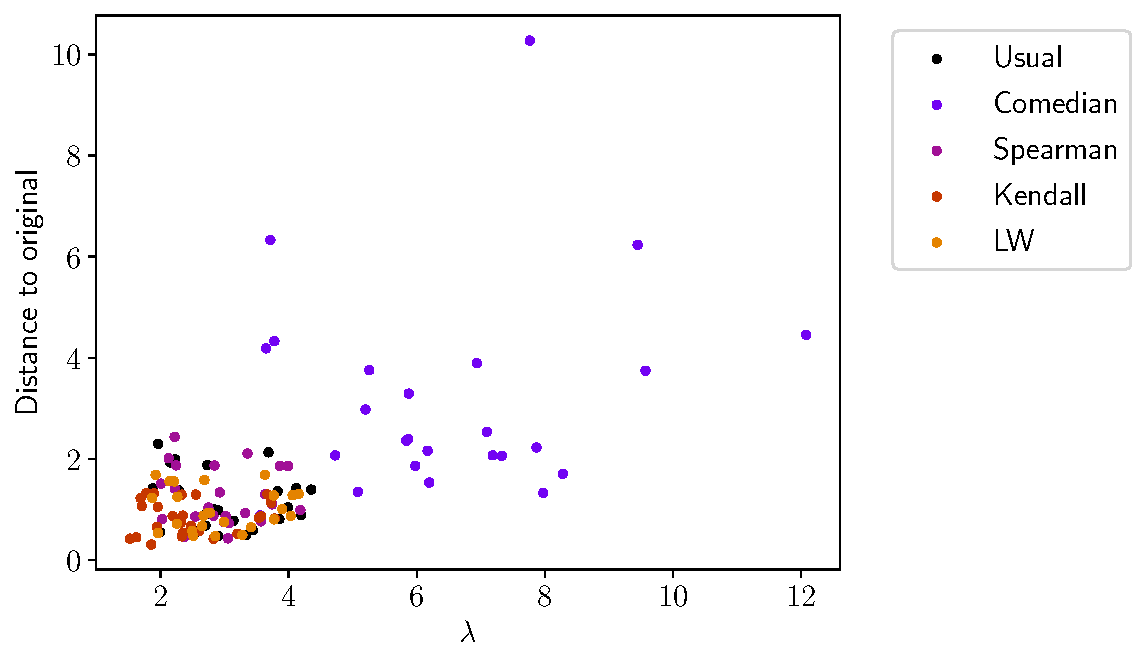
\includegraphics[width=0.8\textwidth]{figs/noise-scatter.pdf}
    \caption{Pareto boundaries for inputs with noise.}
    \label{fig:paretonoise}
\end{figure}

\section{Conclusions}\label{sec:conc}

In conclusion, in first place, faster implementations for the Kendall, Spearman and Comedian matrix estimator were successfully created. These implementations were much faster than the naïve implementations with a big downgrade in memory management. This is deemed by the authors as a worthy tradeoff as memory can be improved with hardware; on the other hand, implementation speeds cannot be massively improved by the same logic. Furthermore, it is important to remark that this implementations are significantly faster because \texttt{for}-loops where avoided and only operations given by the \texttt{numpy} package where used.

In second place, the dissimilarity functions were successfully evaluated. The experiments realized in this work showed that the proposed function by \textcite{tuzel2006} had much better performance than the classic Frobenius norm. This was confirmed by Fig. \ref{fig:linear}, as the linear regression had a $\beta_1 > 1$. Furthermore, this could be justified as covariance matrices do not belong to a euclidean space; hence, the Frobenius dissimilarity could not effectively separate each region.

In third place, the covariance matrices were sucessfully evaluated. The overall best covariance matrix was using the one based on Kendall's tau coefficient. On the other hand, using this covariance estimator yielded a significantly slower execution time (even with the improvement on the implementation). Therefore, the results also showed that the Ledoit-Wolf covariance estimator is the second best algorithm and is much faster. In this manner, both of the mentioned covariance matrices are selected by the authors as the more effective covariances.

For future work, the integral image data structue \parencite{porikli2005integral} could be tested to enhance the speed of the algorithm when exploring the regions of the image.

\printbibliography
\end{document}
